% TBP-double-Ag100
When adsorbed on a (100) silver surface, the molecules arrange in a nice pattern (see figure \ref{fig:two-leg-trans-ag100-motiv}). Although the pattern is dense no problems showed up when designing the molecular models. This is because the last molecules at the perimeter of this island is nicely distinguishable and continuing their regular pattern to the center of the island results in a accurate description of the island.

\begin{figure}[h]
 \centering
 \subfigure[]{
 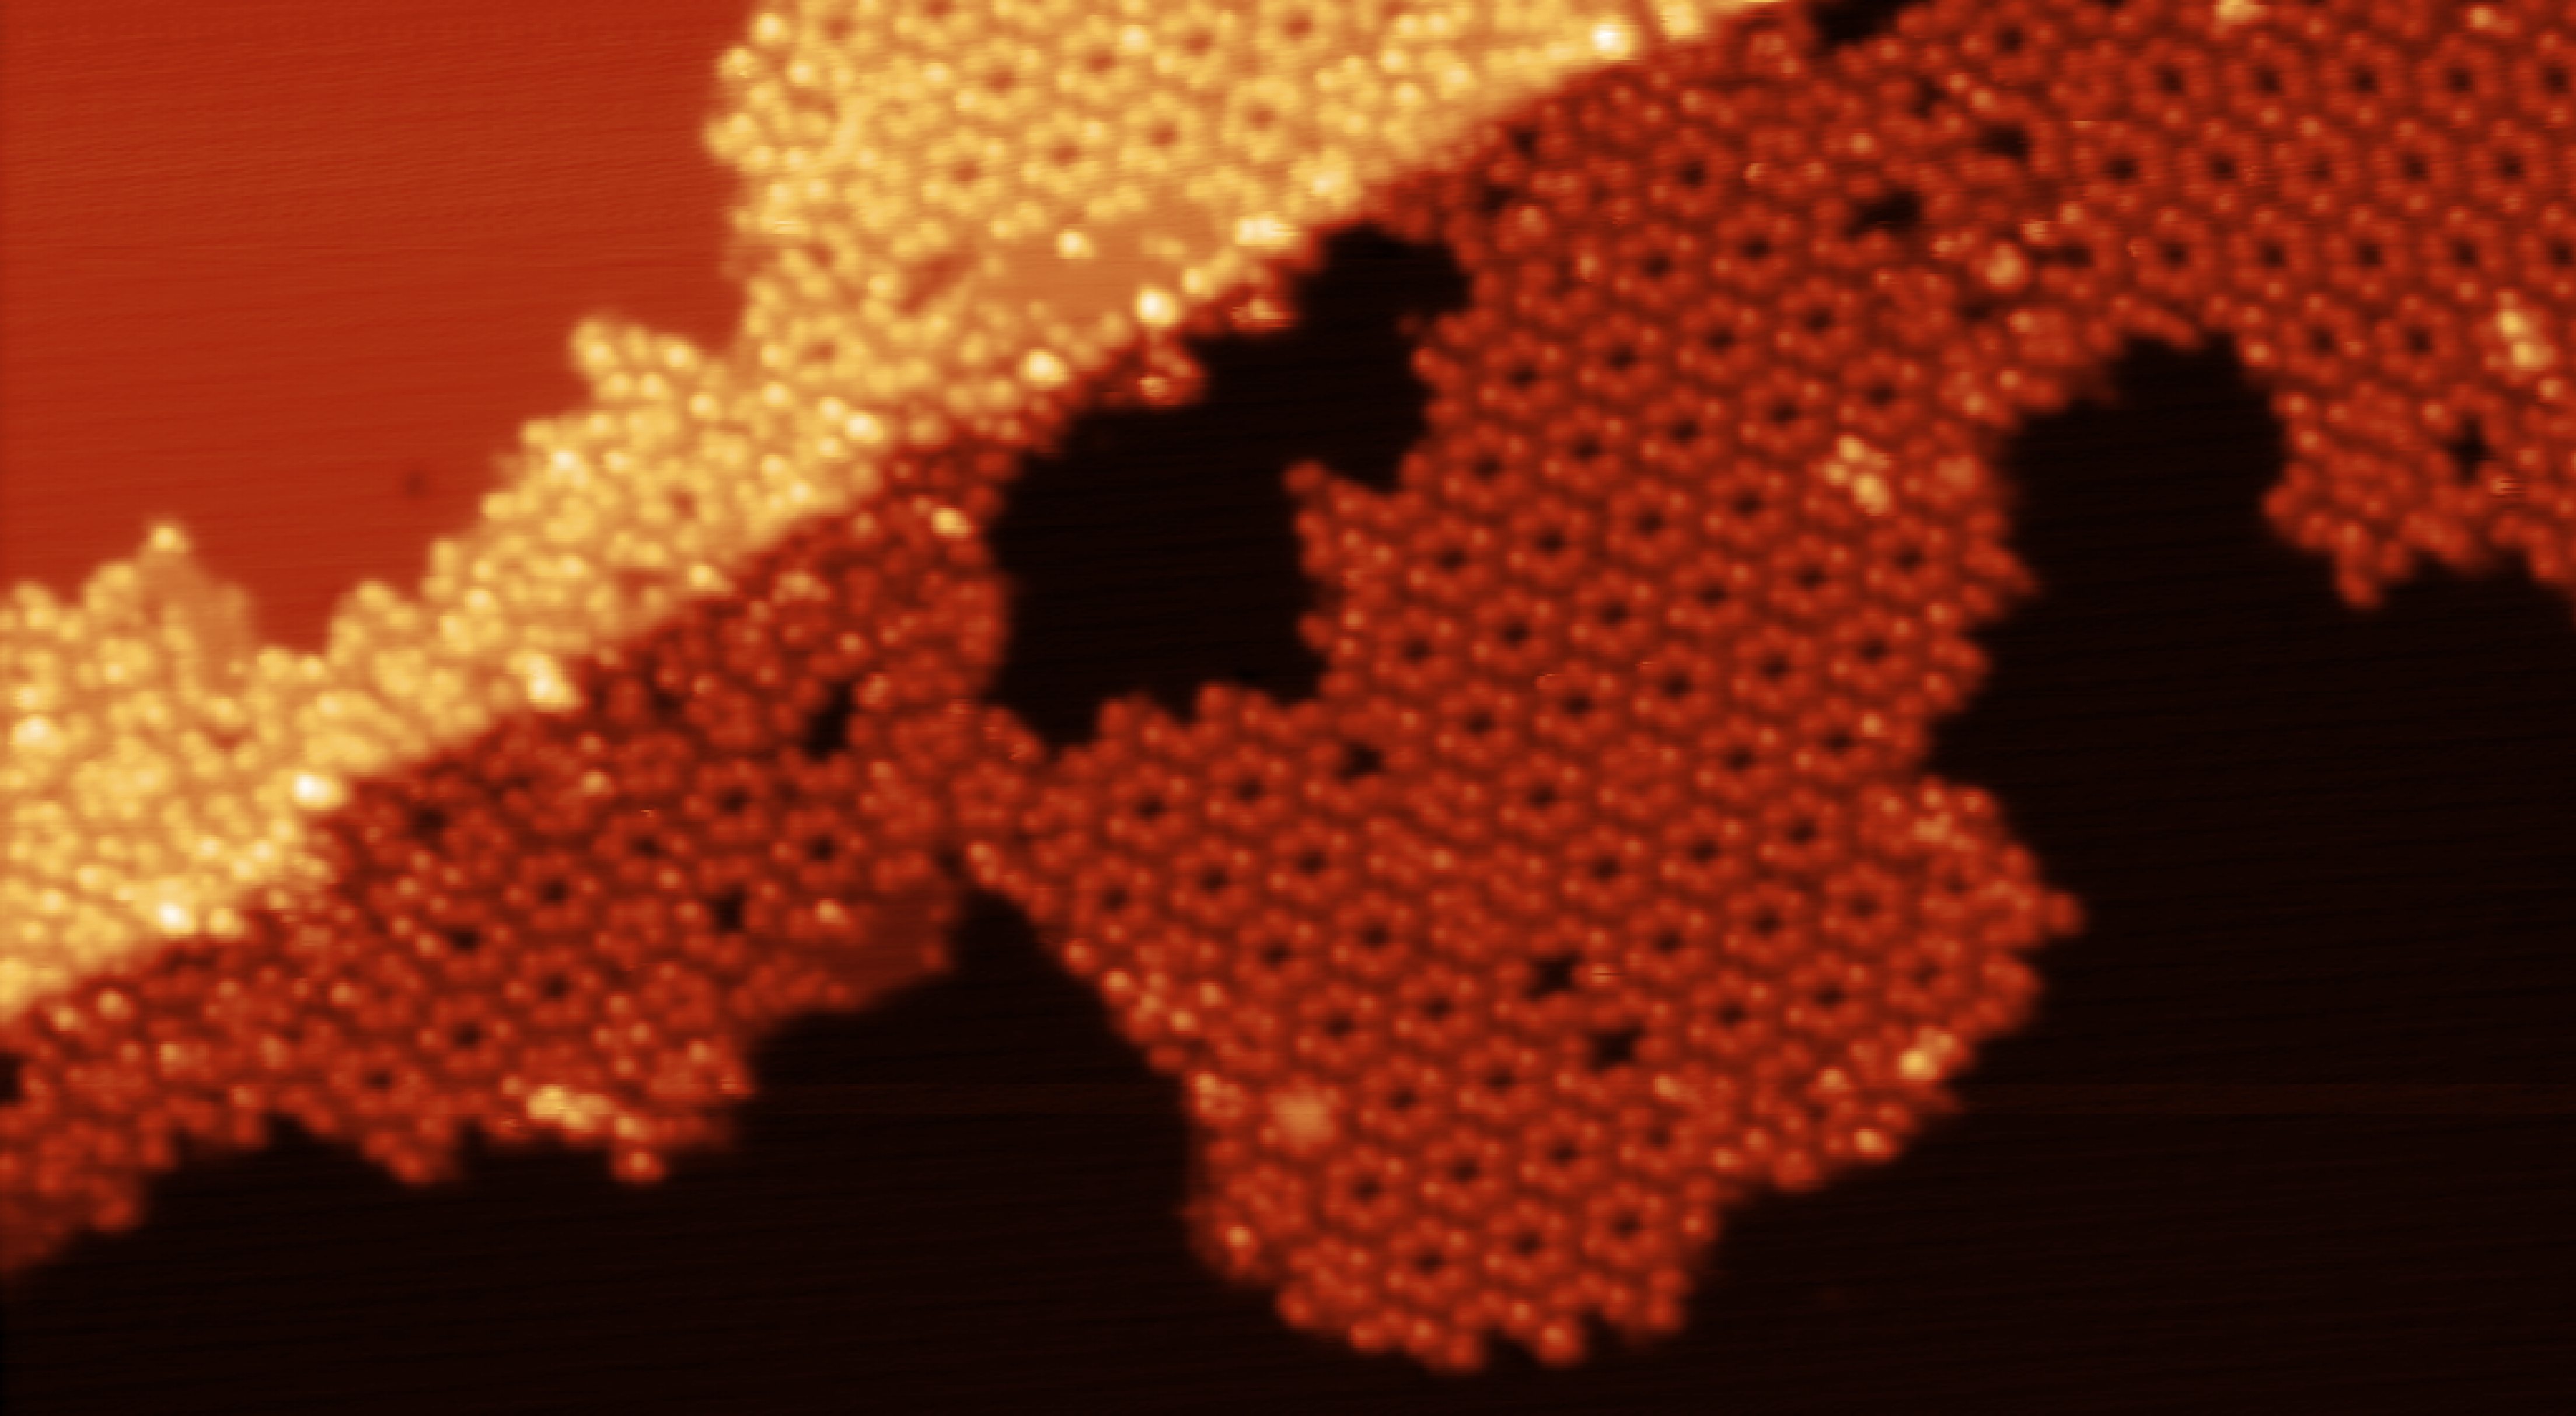
\includegraphics[width=0.70\textwidth]{./images/F160429-172019.png}
} %COARSE MODE!
 \subfigure[\SI{37} x \SI{37}{\nano \meter \squared} patch of self-assembled molecules adsorped at RT]{
 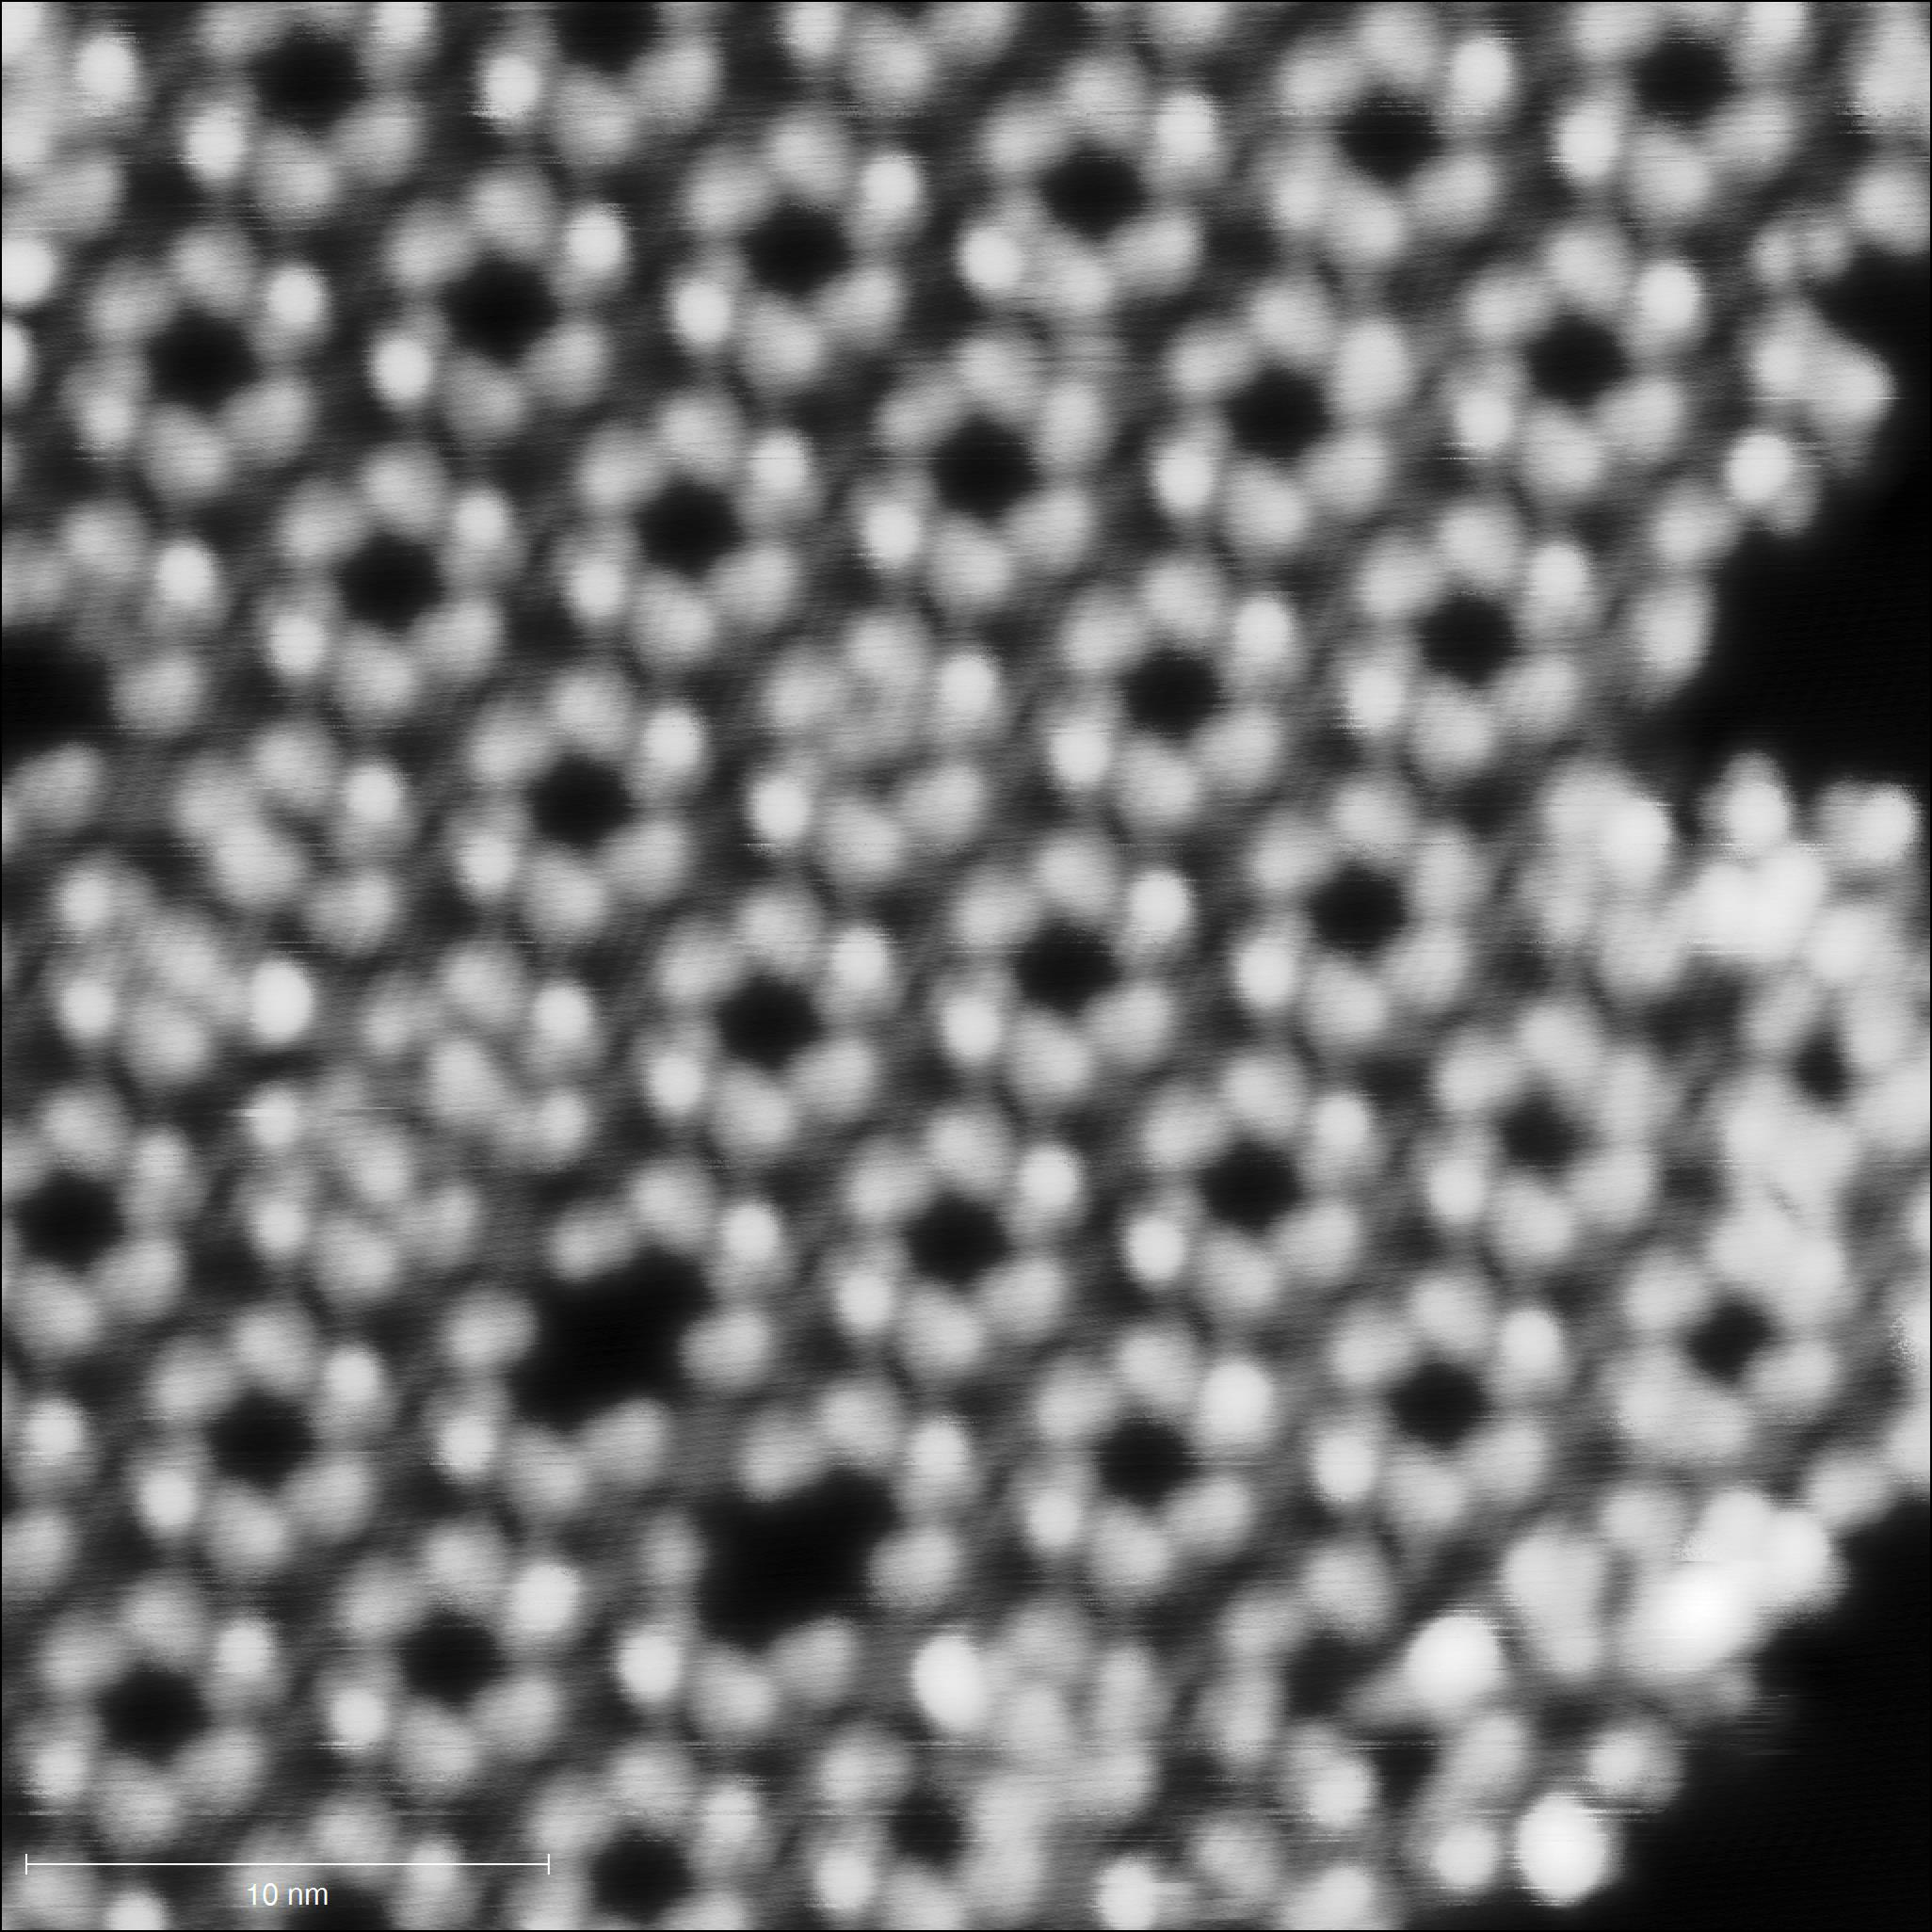
\includegraphics[width=0.3\textwidth]{./images/F160429-185245-R.png}
 } \qquad %COARSE MODE!
 \subfigure[Enlarged view on the unit cells]{
 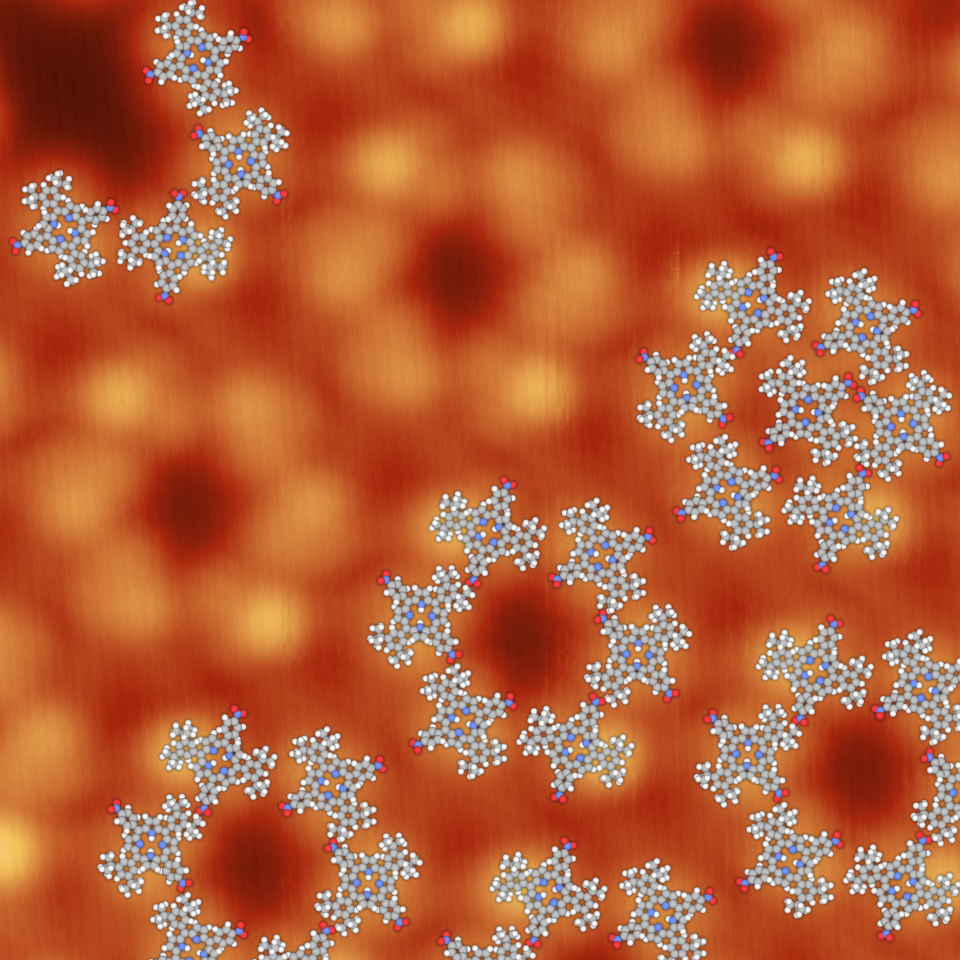
\includegraphics[width=0.3\textwidth]{./images/F160429-185245-R-cut-model.png}
 } %COARSE MODE!
\caption{Trans-TBP adsorped on Ag(100) at room temperature. a) shows a large (37*37nm) fraction of the assembled molecules. The unit cell constituents are enlarged in b) where parts of a) are shown and molecular models overlaid.}
\label{fig:two-leg-trans-ag100-motiv}
\end{figure}